% !TEX root = ../main.tex
%
\chapter{Verwandte Arbeiten}
\label{sec:related}

Die in~\ref{sec:intro:goals} beschriebenen Ziele werden bereits seit langem erforscht.
Der Begriff \textit{Wissensgraph} wurde 2012 durch Google popularisiert, die Ideen dahinter lassen sich allerdings bis ins Ende des 19. Jahrhunderts zurückverfolgen.
Dieses Kapitel zeigt auf, wie sich die Themen dieser Arbeit in die bisherige Forschung einfügen.
\ref{sec:related:kr} ordnet das Konzept des Wissensgraphen in die Entwicklungsgeschichte der Wissensrepräsentation ein.
\ref{sec:related:kbc} beschreibt die aktuell verwendeten Verfahren zur Konstruktion von Wissensgraphen.
In~\ref{sec:related:nlp} wird schließlich ein Überblick über die momentan verbreiteten NLP (\textit{natural language processing}) Werkzeuge gegeben.

\section{Ansätze zur Wissensrepräsentation}
\label{sec:related:kr}

\subsection{Logische Grundlagen}
\label{sec:related:kr:logic}

Die Entwicklung der Wissensrepräsentation hängt eng mit der Entwicklung der Logik zusammen.
Während in der formalen Logik und Mathematik die Prädikatenlogik das allgemein verwendete Kalkül ist und alternative Formalismen kaum verbreitet sind, finden im Bereich der Wissensrepräsentation bis heute diverse andere Kalküle Verwendung.
Diese werden im Folgenden kurz vorgestellt.

\paragraph{Begriffsschrift (1879)}
Gottlob Freges Buch über die \textit{Begriffsschrift} gilt als eines der bedeutsamsten Werke der Logik.
Sie ist der erste Formalismus mit der Mächtigkeit der modernen Prädikatenlogik zweiter Ordnung mit Identität.
Frege benutzt hierfür eine zweidimensionale Notation, die sich stark von der heute gebräuchlichen, linearen, an die Algebra angelehnte Notation unterscheidet.
\begin{equation*}
	\vcenter{\hbox{\Fconditional[\Fanqn{a}]{\Fcontent \mathfrak{R(a)}}{\Fncontent \mathfrak{P(a)}}}}
	\quad\Leftrightarrow\quad \exists\ a: P(a) \lor R(a)
\end{equation*}
Im Gegensatz zur Prädikatenlogik gibt es keine eigene Syntax für \textit{UND} und \textit{ODER};
diese Operatoren müssen durch die Kombination von Negation und Implikation abgebildet werden.
Zudem gibt es ausschließlich den Allquantor;
eine existenzquantisierte Aussage muss durch Negation der negierten allquantisierten Aussage ausgedrückt werden.

\paragraph{Existential Graphs (1882)}
Unabhängig von Frege entwickelte der amerikanische Mathematiker Charles Sanders Peirce ebenfalls ein prädikatenlogisches Kalkül.
Ähnlich wie die Begriffsschrift werden Peirces \textit{Existential Graphs} (zu dt.~Existenzgraphen) zweidimensional dargestellt.
Von dieser Gemeinsamkeit abgesehen, funktionieren sie allerdings fundamental verschieden.
Ein logischer Ausdruck wird hier durch einen ungerichteten Graphen beschrieben.
Die konkrete räumliche Anordnung der Knoten und Kanten hat dabei keine semantische Relevanz.

Peirce hat Existenzgraphen als ein dreistufiges aufeinander aufbauendes System konstruiert.
Die erste Stufe, die sog.\ $\alpha$-Graphen, umfasst alle notwendigen syntaktischen Elemente, um ein Kalkül mit der Mächtigkeit der Aussagenlogik zu erhalten.
Die $\beta$-Graphen bilden die zweite Stufe und erweitern die Syntax der $\alpha$-Graphen, sodass die Mächtigkeit der Prädikatenlogik erster Ordnung erreicht wird.
Sowohl für $\alpha$-, als auch für $\beta$-Graphen, ist die Vollständigkeit und Korrektheit bewiesen.
Die dritte Stufe ($\gamma$-Graphen) wurde von Pierce nie vollendet;
sie deckt in etwa die Mächtigkeit der heutigen Prädikatenlogik höherer Ordnung sowie der Modallogik ab.
\begin{align*}
	\vcenter{\hbox{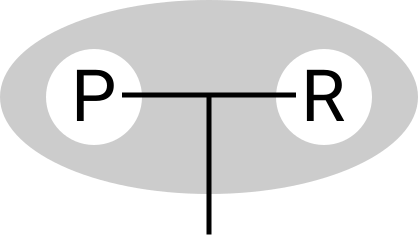
\includegraphics[height=3em]{gfx/related-work/existentialGraphExample1.pdf}}}
	\quad\Leftrightarrow\quad \exists\ a: P(a) \lor R(a)
\end{align*}
Wie schon die Begriffsschrift, sind Existenzgraphen syntaktisch minimal.
Direkt ausdrücken lässt sich lediglich \textit{UND}, der Existenzquantor und die Negation.
Ein weiterer Unterschied zur heutigen Prädikatenlogik ist die Beschreibung logischer Inferenzen.
Im Gegensatz zu den prädikatenlogischen Ersetzungsaxiomen, die auf der syntaktischen Struktur von logischen Ausdrücken operieren (z.~B. für Kommutativität), lassen sich die Ersetzungsaxiome für Existenzgraphen als Graphtransformationsregeln verstehen, die bestimmte Teilmengen der Knoten und Kanten eines Ausdrucks durch andere äquivalente Knoten- und Kantenmengen ersetzen.

\paragraph{Prädikatenlogik (1910)}
Die moderne Notation für prädikatenlogische Ausdrücke lässt sich auf Bertrand Russell und Giuseppe Peano zurückführen.
Die vorherigen zweidimensionalen Schreibweisen wurden häufig kritisiert, da sie die algebraische Notation der symbolischen Logik von Boole und De Morgan verwarfen.
Jene Schreibweisen haben sich daher nicht durchsetzen können.
In den \textit{Principia Mathematica} wird erstmals eine Notation verwendet, die sehr ähnlich zu der heutigen ist.
Ideen, wie Peirces Existenzgraphen, fanden anschließend für mehrere Jahrzehnte kaum Beachtung.

\subsection{Entwicklung maschineller Wissensrepräsentation}
\label{sec:related:kr:history}

\subsubsection{General Problem Solver (1959)}
\label{sec:related:kr:history:gps}

\subsubsection{Expertensysteme (1970)}
\label{sec:related:kr:history:expert}

\subsubsection{Conceptual Graphs (1976)}
\label{sec:related:kr:history:cg}

\subsection{Aktuelle Wissensrepräsentationsansätze}
\label{sec:related:kr:today}

\subsubsection{Semantic Web}
\label{sec:related:kr:today:sw}

\subsubsection{NELL}
\label{sec:related:kr:today:nell}

\subsubsection{Google Knowledge Graph}
\label{sec:related:kr:today:google-kg}

\section{Konstruktionsansätze für Wissensgraphen}
\label{sec:related:kbc}

\section{NLP Werkzeuge}
\label{sec:related:nlp}
